%%%%%%%%%%%%%%%%%%%%%%%%%%%%%%%%%%%%%%%%%
% University/School Laboratory Report
% LaTeX Template
% Version 3.1 (25/3/14)
%
% This template has been downloaded from:
% http://www.LaTeXTemplates.com
%
% Original author:
% Linux and Unix Users Group at Virginia Tech Wiki 
% (https://vtluug.org/wiki/Example_LaTeX_chem_lab_report)
%
% License:
% CC BY-NC-SA 3.0 (http://creativecommons.org/licenses/by-nc-sa/3.0/)
%
%%%%%%%%%%%%%%%%%%%%%%%%%%%%%%%%%%%%%%%%%

%----------------------------------------------------------------------------------------
%	PACKAGES AND DOCUMENT CONFIGURATIONS
%----------------------------------------------------------------------------------------

\documentclass{article}

\usepackage[version=3]{mhchem} % Package for chemical equation typesetting
\usepackage{siunitx} % Provides the \SI{}{} and \si{} command for typesetting SI units
\usepackage{graphicx} % Required for the inclusion of images
\usepackage{natbib} % Required to change bibliography style to APA
\usepackage{amsmath} % Required for some math elements 
\usepackage{caption}
\usepackage{subcaption}

\setlength\parindent{0pt} % Removes all indentation from paragraphs

\renewcommand{\labelenumi}{\alph{enumi}.} % Make numbering in the enumerate environment by letter rather than number (e.g. section 6)

%\usepackage{times} % Uncomment to use the Times New Roman font

%----------------------------------------------------------------------------------------
%	DOCUMENT INFORMATION
%----------------------------------------------------------------------------------------

\title{Stat 133\\ BML Traffic Model Simulation} % Title

\author{HungWei \textsc{Lin}} % Author name

\date{\today} % Date for the report

\begin{document}

\maketitle % Insert the title, author and date


% If you wish to include an abstract, uncomment the lines below
% \begin{abstract}
% Abstract text
% \end{abstract}

%----------------------------------------------------------------------------------------
%	SECTION 1
%----------------------------------------------------------------------------------------

\section{BML Simulation Study}

I choose my grid size to be 64 by 64.

\begin{enumerate}
\begin{item}
For what values of p, the density of the grid, did you find free flowing traffic and traffic jams? Did you find any cases of a mixture of jams and free flowing traffic?

Ans: In my simulation, p is around 0.3 to 0.4 because when $p>=0.5$, the grids tend to be blocked.
\end{item}

\begin{item}
How many simulation steps did you need to run before observing this behavior?

Ans: I choose simulation steps to be 1000 because when $p>=0.5$, the grids are almost always blocked within 1000 steps. (See Figure 2)

\end{item}
\begin{item}
Does the transition depend on the size or shape of the grid?

Ans: It depends on the shape of the grid because one can easily make a blocked matrix by manually placing the red and blue cars; however, in my observation, the transition does not really depend on the size of the grid because when I ran large matrices, critical density is about 0.3 to 0.4 as well. Thus, I believe that the transition depends on the density of the grids.
\end{item}
\end{enumerate}

 
%----------------------------------------------------------------------------------------
%	SECTION 2
%----------------------------------------------------------------------------------------

\section{Simulation Data and Graphs}


\begin{figure}
        \centering
        \begin{subfigure}[b]{0.3\textwidth}
                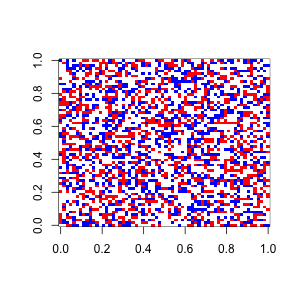
\includegraphics[width=\textwidth]{example001}
                \caption{Initial Matrix}
        \end{subfigure}
        \begin{subfigure}[b]{0.3\textwidth}
                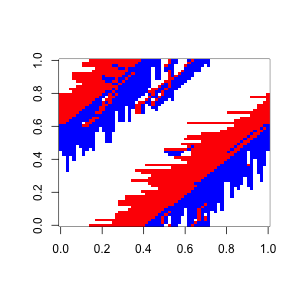
\includegraphics[width=\textwidth]{example002}
                \caption{After 251 Steps}
        \end{subfigure}
        \caption{64 by 64 matrix with p=0.5}
\end{figure}


\begin{figure}[h]
\begin{center}
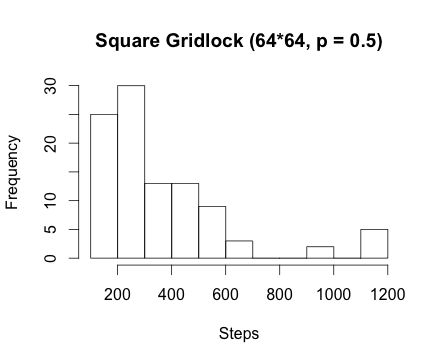
\includegraphics[width=0.65\textwidth]{gridlockhist} 
\caption{Distribution of A hundred 64 by 64 Matrices. \\
About ninty-five of them are blocked within 1000 Steps}
\end{center}
\end{figure}






\end{document}